% Figura cuerpo B3 (4.2.2): el canal del margen contracíclico en el mercado de trabajo
\documentclass[tikz,border=3pt]{standalone}
\usepackage[T1]{fontenc}
\usepackage[utf8]{inputenc}
\usepackage{amsmath}
\usetikzlibrary{arrows.meta,calc,positioning}
\begin{document}
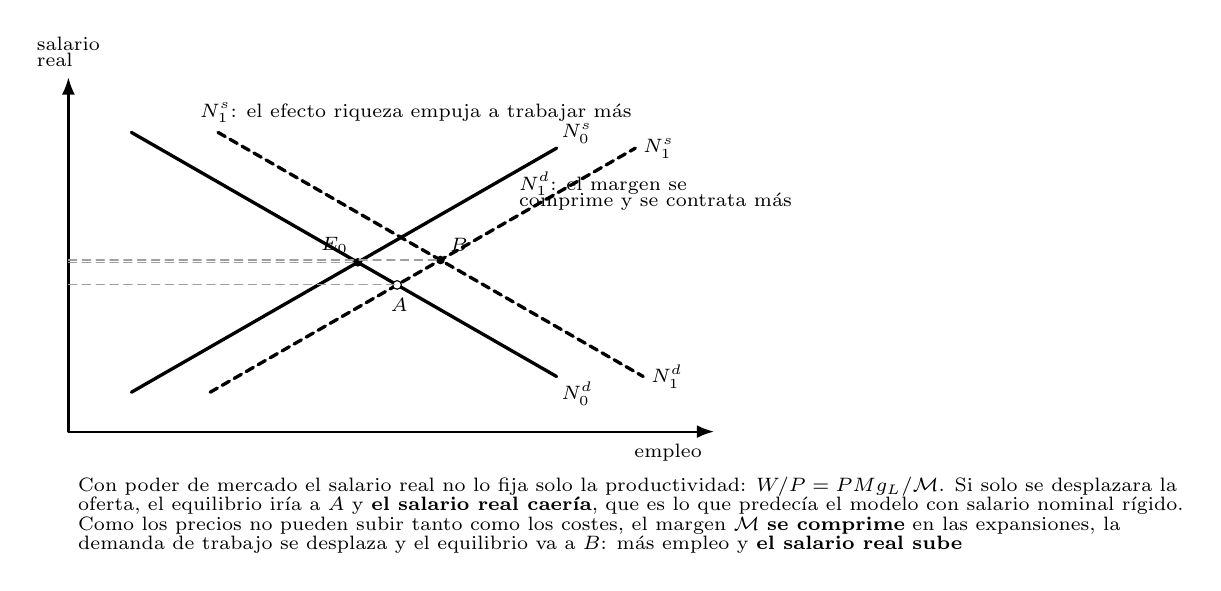
\begin{tikzpicture}[>={Latex[length=2.2mm]}, line cap=round, font=\footnotesize,
  eje/.style={->, thick},
  curva/.style={very thick},
  nueva/.style={very thick, densely dashed},
  guia/.style={densely dashed, gray!75},
  pto/.style={circle, fill=black, inner sep=1.1pt},
  contra/.style={circle, draw=black, fill=white, inner sep=1.1pt}]

  \draw[eje] (0,0) -- (8.2,0) node[below left=1pt, font=\scriptsize]{empleo};
  \draw[eje] (0,0) -- (0,4.5) node[above, font=\scriptsize, align=left]{salario\\[-2pt]real};

  \draw[curva] (0.8,0.50) -- (6.2,3.60) node[above right=-3pt, font=\scriptsize]{$N^{s}_{0}$};
  \draw[nueva] (1.8,0.50) -- (7.2,3.60) node[right=-1pt, font=\scriptsize]{$N^{s}_{1}$};
  \draw[curva] (0.8,3.80) -- (6.2,0.70) node[below right=-3pt, font=\scriptsize]{$N^{d}_{0}$};
  \draw[nueva] (1.9,3.80) -- (7.3,0.70) node[right=-1pt, font=\scriptsize]{$N^{d}_{1}$};

  \node[pto] (E0) at (3.674,2.150) {};
  \node[anchor=south east, inner sep=2pt, font=\scriptsize] at (3.63,2.19) {$E_{0}$};
  \node[contra] (A) at (4.174,1.863) {};
  \node[anchor=north, inner sep=3pt, font=\scriptsize] at (4.20,1.80) {$A$};
  \node[pto] (B) at (4.725,2.179) {};
  \node[anchor=south west, inner sep=2pt, font=\scriptsize] at (4.77,2.21) {$B$};

  \draw[guia] (0,2.150) -- (3.674,2.150);
  \draw[guia] (0,1.863) -- (4.174,1.863);
  \draw[guia] (0,2.179) -- (4.725,2.179);

  \node[anchor=west, font=\scriptsize, align=left] at (1.55,4.05)
    {$N^{s}_{1}$: el efecto riqueza empuja a trabajar más};
  \node[anchor=west, font=\scriptsize, align=left] at (5.6,3.05)
    {$N^{d}_{1}$: el margen se\\[-2pt]comprime y se contrata más};

  \node[align=left, anchor=north west, font=\scriptsize] at (0,-0.45)
    {Con poder de mercado el salario real no lo fija solo la productividad: $W/P=PMg_{L}/\mathcal{M}$. Si solo se desplazara la\\[-1pt]oferta, el equilibrio iría a $A$ y \textbf{el salario real caería}, que es lo que predecía el modelo con salario nominal rígido.\\[-1pt]Como los precios no pueden subir tanto como los costes, el margen $\mathcal{M}$ \textbf{se comprime} en las expansiones, la\\[-1pt]demanda de trabajo se desplaza y el equilibrio va a $B$: más empleo y \textbf{el salario real sube}};
\end{tikzpicture}
\end{document}
